\documentclass[10pt]{article}
%\documentclass[9pt]{extarticle}

% Handle enumeration list
\usepackage{enumitem}

% Citations as footnotes
% \usepackage[style=verbose,backend=bibtex]{biblatex}
% \bibliography{refs.bib}

\usepackage{amsmath}
\usepackage{amssymb}
\usepackage{graphicx}
\usepackage{microtype}

% Directory for images
\graphicspath{{images/}}

% To wrap text around figures
\usepackage{wrapfig}
\usepackage{caption}

% Define new type of columns
\usepackage{array}
\usepackage{tabulary}
\newcolumntype{K}[1]{>{\centering\arraybackslash}m{#1}}

% Stretch the dimension of the rows in tables
\renewcommand{\arraystretch}{1.6}

% Add colors to table
\usepackage{colortbl}

% Set Helvetica as main font
\usepackage{helvet}
\renewcommand\familydefault{\sfdefault}
\usepackage[T1]{fontenc}

% Set Helvetica as main font for equations
\usepackage[helvet]{sfmath}

% Change geometry of the page
\usepackage[margin=1in]{geometry}

\usepackage[svgnames]{xcolor}
\usepackage[hidelinks]{hyperref}

\usepackage{multicol}

% Redefine names
\newcommand{\sectionname}{Section}
\renewcommand{\appendixname}{Appendix}
\newcommand{\equationname}{Equation}
\newcommand{\referencename}{Ref.}
\renewcommand{\figurename}{Figure}
\renewcommand{\tablename}{Table}

% Some useful definition
\newcommand{\DW}{D-Wave 2X}

\begin{document}

\begin{center}\Large
\textbf{Quantum Annealing for Air Traffic Management\\Interim Report, July 2016\\Quantum AI Lab, NASA Ames}
\end{center}

\begin{multicols}{2}
%\begin{center}
\colorbox{gray!20}{
  \begin{minipage}[t]{0.9\columnwidth}
    \textbf{Summary of completed tasks (3.5 Months):}
      \begin{itemize}[leftmargin=0.5cm]
        \itemsep-0.5em
        \item Devised code to analyze wind-optimal trajectories.
        \item Identified all the potential conflicts.
        \item Developed a formulation of the problem amenable to expressing as QUBO.
        \item Developed a mapping of the problem without maneuvers to QUBO.
      \end{itemize}
    \textbf{Next steps (remaining 8.5 months):}
      \begin{itemize}[leftmargin=0.5cm] 
        \itemsep-0.5em
        \item Develop a variety of mappings to QUBO of the problem with maneuvers.
        \item Identify a set of benchmark ATM problems.
        \item Analyze the performance of state-of-art classical QUBO solvers on the benchmark set.
        \item Analyze the performance of the \DW chip on the benchmark set.
        \item Compare classical and quantum performance.
        \item Explore scalability on future hardware and architectures.
      \end{itemize}
 \end{minipage}
}
\end{center}

%\section*{Introduction}\label{sec:intro}
Building on our promising prior results in the planning domain~\cite{rieffel:15,venturelli:15},
we have begun to explore the potential of quantum annealing (QA) for solving challenging computational problems related to air traffic management (ATM)\cite{rodionova:16, rodionova:thesis15}.
This work is being performed by members of the QuAIL team (Tobias Stollenwerk, Bryan O'Gorman, Salvatore Mandr\`a, Davide Venturelli and Eleanor G. Rieffel) with expertise in all aspects of applying quantum annealing to real-world problems, in close collaboration with domain experts in ATM (Olga Rodionova, Hok K. Ng and Banavar Sridhar).
We have identified a specific problem within ATM to serve as a case study, and have made significant progress towards formulating it in a way that is amenable to quantum computing.
See \tablename~\ref{table:milestone} for a complete overview of completed and future milestones.

% \section*{Project Aims and Approach}\label{sec:intro}
% The aim of this project is 
\noindent
{\bf Aim:} To provide an initial assessment of the potential 
of quantum annealing to attack challenging computational problems in the ATM 
domain. 
\linebreak
{\bf Approach:} This assessment will be based on a case study, involving runs
on the \DW\ quantum annealer and classical annealing simulations, in which 
a variety of quantum annealing approaches are developed and compared 
on benchmark problems derived from a specific real-world ATM problem.
\linebreak
{\bf Personnel:} This work is being performed by members of the QuAIL team (Tobias Stollenwerk, Bryan O'Gorman, Salvatore Mandr\`a, Davide Venturelli and Eleanor G. Rieffel) with expertise in applying quantum annealing to real-world problems, in close collaboration with ATM domain experts (Olga Rodionova, Hok K. Ng and Banavar Sridhar).
This work builds on the team's promising prior results in other planning and
scheduling domains~\cite{rieffel:15,venturelli:15}.
% See \tablename~\ref{table:milestone} for a complete overview of completed and future milestones.
\noindent
\begin{minipage}[t]{0.9\columnwidth}
\textbf{Projected final project outputs:}
\begin{itemize}[leftmargin=0.5cm]
  \itemsep-0.5em
  \item Programming toolkit to analyze trajectories and potential conflicts
  \item Mappings of the ATM problem to QUBO
  \item Implemented mappings on benchmark problems: taking a set of wind-optimal trajectories and outputting a QUBO instance
  \item Analysis of runs of benchmark instances on the \DW\ quantum annealer 
  \item Report summarizing initial assessment, with recommendations
for future research
\end{itemize}
\end{minipage}

\subsection*{Results to date (3.5 months)}

\begin{center}
\colorbox{green!10}{
  \begin{minipage}[t]{0.9\columnwidth}
    \textbf{Summary of completed tasks (3.5 Months):}
      \begin{itemize}[leftmargin=0.5cm]
        \itemsep-0.5em
	\item Identified specific ATM problem, deconflicting trajectories, as case study
        \item Devised code to analyze and visualize wind-optimal trajectories
        \item Identified and characterized all potential conflicts in NAT dataset
        \item Developed formulations of a simpler version of the problem 
with only origination delays, amenable being run on a quantum annealer. Write-up available
        \item Began developing formulations that support manoevers as well
as delays
	\item Identified subsets of data treatable independently, a
first step in the design of a set of small benchmark problems
      \end{itemize}
 \end{minipage}
}
\end{center}


We have identified a specific ATM domain to serve as a case study, 
namely deconflicting wind-optimal aircraft trajectories. We build on
the work of Rodionova et al.~\cite{rodionova:16, rodionova:thesis15}
who developed a non-quantum approach to this problem. The following
graphic shows the main steps in developing a quantum annealing approach 
to these problems. 
\begin{minipage}[c]{\columnwidth}
\centering
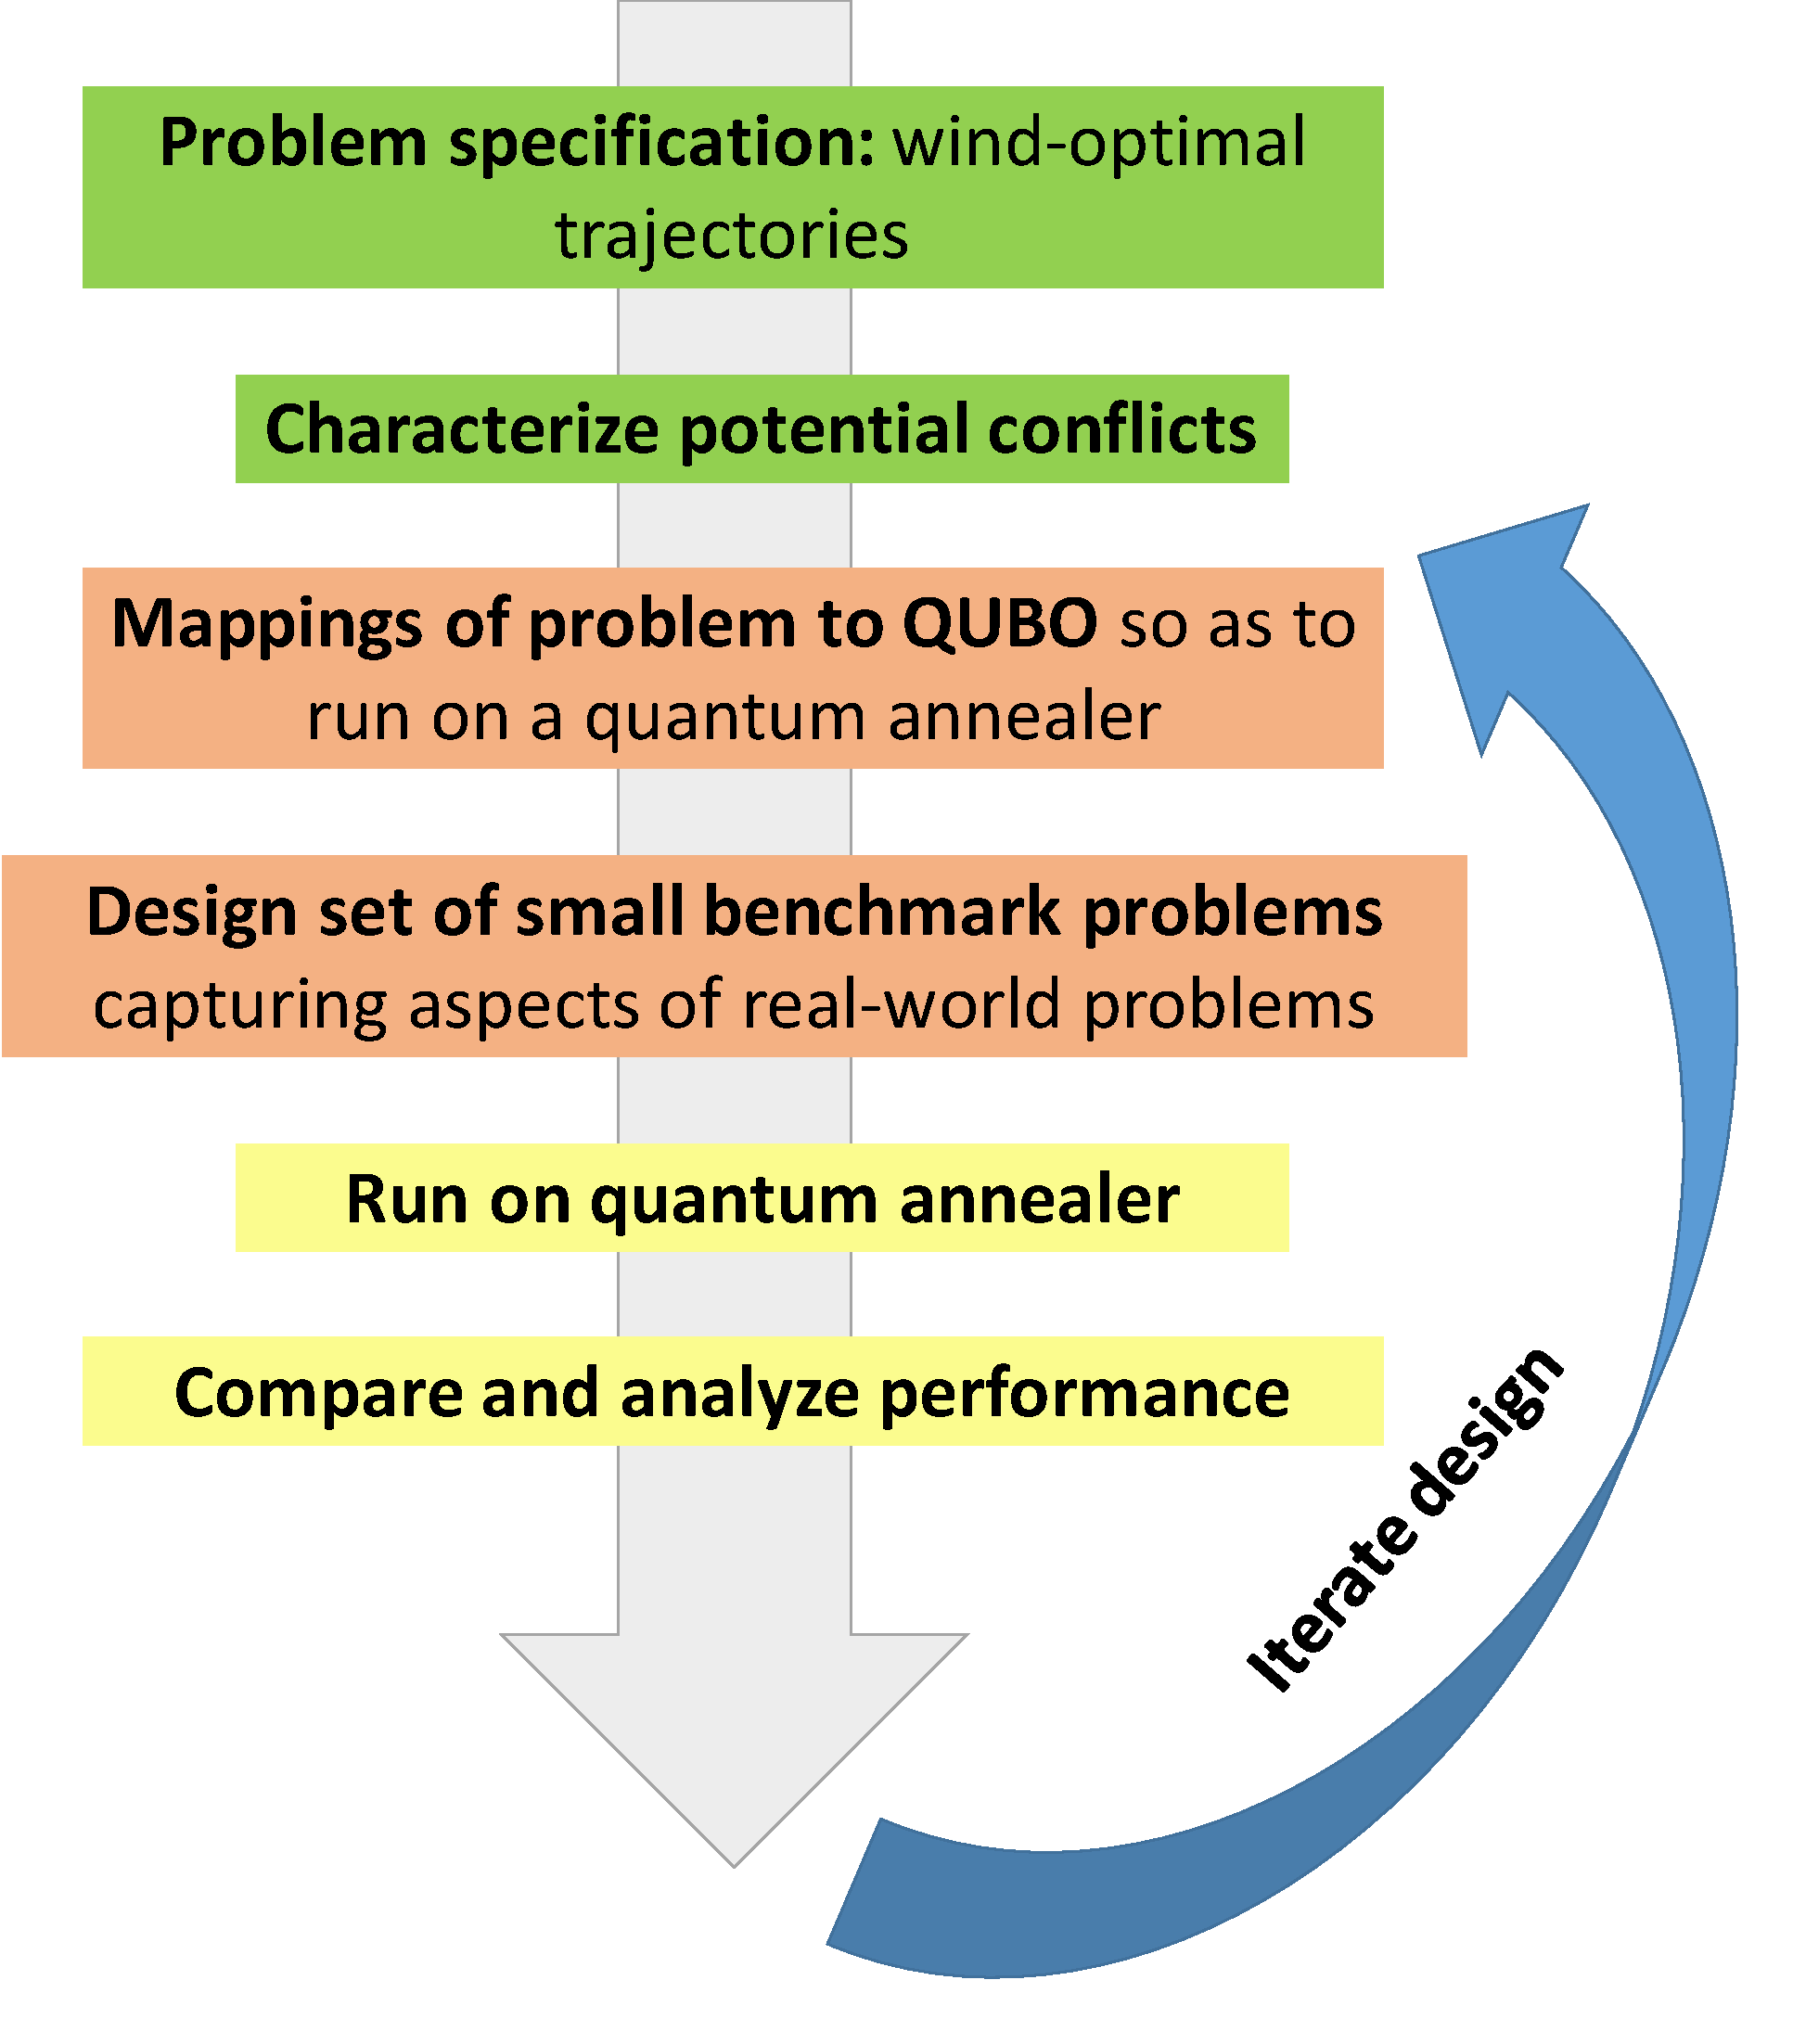
\includegraphics[width=0.8\columnwidth]{flowDiagram}
% \captionof{figure}{Schematic flow diagram to optimize ATM problems using quantum optimizers. Green/light-gray and orange/dark-gray boxes represent respectively completed and partially completed tasks.}
\label{fig:scheme}
\end{minipage}
Throughout this document, green indicates steps
completed in the past 3.5 months, yellow/orange
indicate steps to be completed in the next 4 month period, with orange 
for already partially completed tasks. 
% Uncolored items will be completed within the final 4.5 month stage of the project.

We have formulated a basic version of the problem, one that considers only
origination delays, in a way that is amenable
to quantum computing. Furthermore, we have developed tools to 
characterize the potential
conflicts in order to devise parameterizations and encodings 
of manoevers in flight so that our approach can support quantum annealing
approaches that consider manoevers as well as delays. 
From these formulations, we have developed multiple mappings to 
quadratic unconstrained binary optimization (QUBO), the type of problem
specification current annealers such as the \DW\ require. 

In order to optimize our formulation of the problem for realistic data, we focus
on flight data in the North Atlantic oceanic airspace (NAT). 
Rodionova provided us with
wind-optimal trajectories for two consecutive days (July
28\textsuperscript{th}-29\textsuperscript{th} 2012), trajectories on which her
state-of-the-art approach has been evaluated. 
We have already implemented the first step in processing the raw data
into useful form: given the trajectories, find the set of potential 
conflicts.
We have also developed code to evaluate the dependencies in the data set,
enabling the identification of subsets of the data that can
be treated independently, a step toward the design of suitably small 
benchmark sets that will fit on the \DW\ prototype quantum annealer in spite
of its limitations in terms of number of qubits and connectivity.

% \section*{Formulation of the problem}\label{sec:approach}

Specifically, we are focusing on the problem of minimizing the total delay of a set of flights (each consisting of an origin, destination, and departure time).
More precisely, we are given the wind-optimal trajectories for every flight, and wish to choose a set of modifications of these trajectories so that they a) do not conflict with each other, and b) minimize the sum of the delays of the flights at their destinations, relative to the wind-optimal trajectories.
The main challenge of applying quantum annealing to a real-world problem is in formulating the problem as Quadratic Unconstrained Binary Optimization (QUBO), i.e.\ a quadratic real-valued polynomial over Boolean-valued variables.
To do so, we first had to parameterize the trajectory modifications in such a way that a) the parameterizations could be encoded in Boolean-valued variables, and b) the constraints and cost function (total delay) could be expressed as quadratic polynomial over those bits.
The modifications to the trajectories that we consider are of two types. 
First, we consider origination delays, in which the departure of the flight from its origin is simply delayed, and its trajectory translated in time only. 
Second, we consider avoidance maneuvers, in which flights may briefly change course in order to avoid conflicts with others;
a maneuver is local, and can only change the subsequent part of the trajectory by pushing it forward in time.

\begin{minipage}[c]{\columnwidth}
\centering
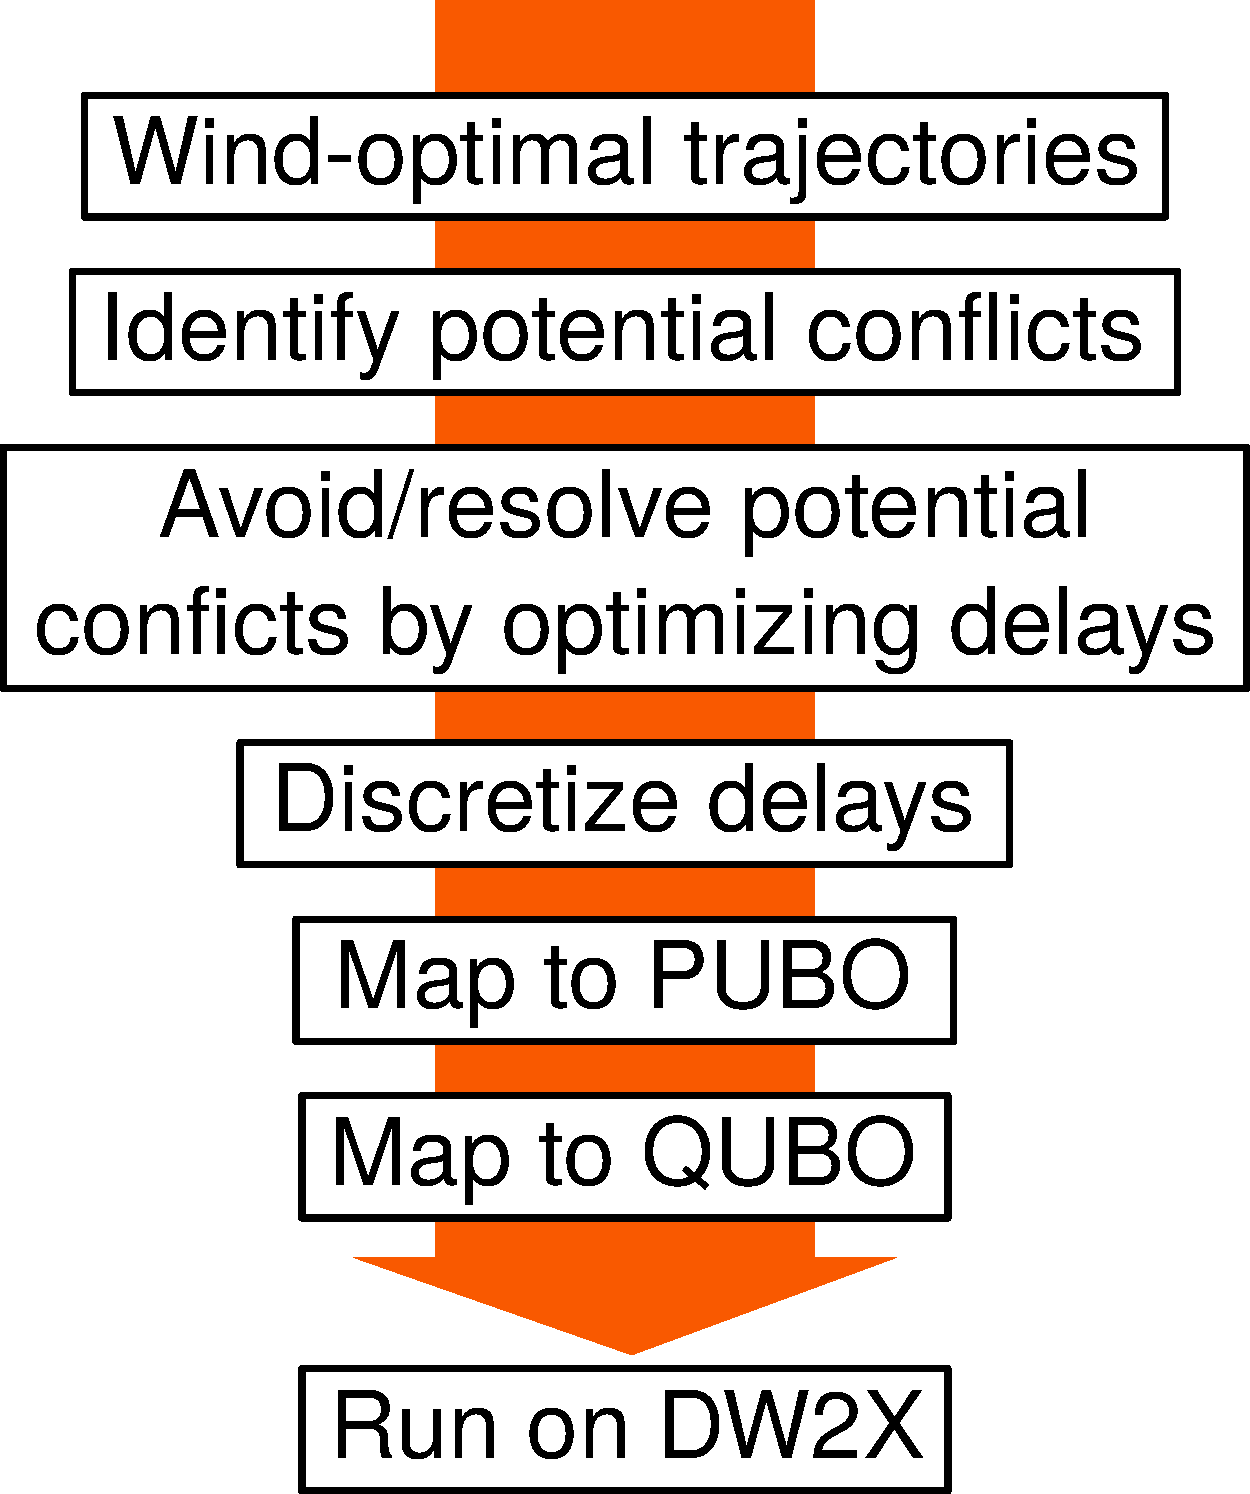
\includegraphics[width=0.7\columnwidth]{scheme}
\captionof{figure}{Schematic flow diagram to optimize ATM problems using quantum optimizers. Green/light-gray and orange/dark-gray boxes represent
respectively completed and partially completed tasks.}
\label{fig:scheme}
\end{minipage}

Given the set of wind-optimal trajectories, we refer to the points in space that more than one trajectory crosses at some time ``spatial conflicts''.
These serve as a starting point in that they allow us to discretely identify potential conflicts.
This allows us to parameterize the modified trajectories by the times at which every flight arrives at its potential conflicts.
Let let $t_{i,k}$ be the variable indicating the time at which flight $i$ gets to potential conflict $k$, and let $t_{i,k}^*$ be the wind-optimal value.
The difference between them $D_{i,k} = t_{i,k} - t^*_{i,k}$ is the accumulation of delays that flight $i$ encounters before conflict $i$.
Let $d_{i,k}$ be the variable indicating the delay added to flight $i$ at potential conflict $k$.
Then the delay can be written $D_{i,k} = d_i + \sum_{k' \in P_{i,k}} d_{i,k}$, where $d_i$ is the origination delay and $P_{i,k}$ is the set of potential conflicts that flight $i$ encounters prior to $k$.
Actual conflicts, i.e.\ when $|t_{i,k} - t_{j,k}|$ is below some threshold $\theta$ for two flights $i$ and $j$ at potential conflict $k$, must be penalized.
For example, this can be done by encoding each time $t_{i,k} = \sum_{\alpha} \alpha t_{i,k,\alpha}$ using bits indicating its value from a discrete set $\{\alpha\}$, and adding the penalty term $\sum_{|\alpha - \beta| < \theta} t_{i,k,\alpha} t_{j,k,\beta}$.
We are currently exploring the relative advantages of encoding the trajectories using the absolute times $\{t_{i,k}\}$ or the relative delays $\{d_{i,k}\}$ (both lead to qualitatively similar resource requirements), as well as different ways of encoding the potential maneuvers, especially when multiple flights potentially conflict at the same point in space and time.
The inclusion of maneuvers leads to higher-degree terms in the cost function.
We will try two approaches to address this: first, using standard locality-reduction gadgets~\cite{babbush:13}, which requires extra ancillary bits; and second, using Lagrange multipliers~\cite{ronagh:15} to enforce the constraints from which the higher-degree terms arise.

%\section*{Implementation and benchmarks}

In order to optimize our formulation of the problem to realistic data, we focus
on flight data in the North Atlantic oceanic airspace (NAT), for which we have
wind-optimal trajectories for two consecutive days (July
28\textsuperscript{th}-29\textsuperscript{th} 2012) for which state-of-the-art
solutions exist.  The NAT dataset consists of wind-optimal trajectories in
(3+1)-dimensions for 984 flights. 
These trajectories, subsets thereof, and toy-instances based thereon will serve as our benchmark set.

\indent We have already implemented the first step in processing the raw data
into a useful form: given the trajectories, finding the set of potential
conflicts.  Using additional tools also already developed, we are currently
looking closely at these potential conflicts in order to devise
parameterizations and encodings of possible maneuvers that are amenable to a
QUBO formulation.
Importantly, our ASD collaborators have already expressed interest in the visualization tools we have developed, an excellent example of how work such can have benefits beyond quantum annealing.

%\section*{Outlook and next steps}\label{sec:ass}

Already we have formulated the ATM problem in a way that is amenable to pseudo-Boolean optimization.
Our next step is to finalize the mappings to QUBO, and assess the quality of solutions from the resulting QUBO instances to those found by prior classical methods, based on ATM instances drawn from the NAT dataset.
That is, before we analyze the performance of quantum annealing in solving our formulation of the problem, we will analyze the formulation itself, by comparing solutions from classical QUBO solvers to those from extant methods.
We are interested not only in solutions that are at least as good in quality, but those that are of at least similar quality but sufficiently different from those produced by other methods; in computational models of real-world problems such as this, there is a wide-ranging interest in a \emph{diversity} of solutions from which a human can select based on unformalized criteria.

We will also construct small instances, either derived directly from subsets of the NAT dataset or based on the structures therein, and run them both on a physical state-of-the-art D-Wave quantum annealer as well as a simulation of quantum annealer, which allows for larger sizes in order to asses the scalability of our methods.
Finally, we will explore the resource requirements of various mappings for realistic data in order to direct future hardware designs.
These last steps encompass the motivating premise of this work: that by formulating computational problems of interest to NASA in a way that is amenable to quantum annealing, we can set the stage for both directing and utilizing the development larger-scale quantum annealers.

% For a complete overview of completed tasks and future milestones, see \tablename~\ref{table:milestone}.
% \figurename~\ref{fig:scheme} summarizes the steps involved in applying quantum annealing to the ATM problem.

\subsection*{Proposed next steps (4 months)}\label{sec:ass}

We need to finalize the mappings to QUBO for the full problem,
supporting both origination delays and in-flight manoevers.
We will design benchmark small instances, either well-chosen subsets of 
% the NAT dataset
or constructed instances based on NAT dataset structures. 
Before analyzing the performance of quantum annealing on our
formulation of the problem, we first analyze the formulation itself by
comparing solutions from classical QUBO solvers to those from extant methods.
Then, we run these benchmark instances on the \DW, a
state-of-the-art quantum annealer, and also 
run classical annealing methods on the Pleiades supercomputer 
to support larger size problem, enabling an assessment of 
the scalability of our methods.  
We compare the diversity of solutions returned,
as well as the quality of solutions 
returned,
since in a wide range of settings, practitioners are interested in 
a \emph{diversity} of
solutions from which a human can select based on unformalized criteria.

% This work will put is in a good position to iterate on our parameterizations and encodings in the final 4 months of the year-long project, and to explore the resource requirements of the mappings for realistic data. This final stage will enable us to make an initial assessment of the potential of quantum annealing for this domain, to direct future quantum annealing  hardware designs, establish quantum annealing best practice in this domain.  
% These last steps encompass the motivating premise of this work: that by formulating computational problems of interest to NASA in a way that is amenable to quantum annealing, we can set the stage for both directing and utilizing the development larger-scale quantum annealers.  
\begin{center}
\colorbox{yellow!10}{
  \begin{minipage}[t]{0.9\columnwidth}
    \textbf{Next steps (4 months):}
      \begin{itemize}[leftmargin=0.5cm] 
        \itemsep-0.5em
        \item Develop a variety of mappings to QUBO of the problem with maneuvers.
        \item Design a set of benchmark ATM problems based on NAT data.
        \item Run state-of-art classical QUBO solvers and
the \DW\ quantum annealer on the benchmark set, and analyze the performance.
	\item Feedback results from these initial runs into proplem parameters and encodings. Design more advanced set of quantum annealing or hybrid 
quantum-classical approaches to these problems
      \end{itemize}
 \end{minipage}
}
\end{center}


Request: 150K for \~ 1.5 WYE for 4 months

% For a complete overview of completed tasks and future milestones, see \tablename~\ref{table:milestone}.
% \figurename~\ref{fig:scheme} summarizes the steps involved in applying quantum annealing to the ATM problem.

\begin{table}[h!]\centering
  \begin{tabular}{|m{7cm}|m{7cm}|K{2.8cm}|}
    \rowcolor{gray!30}
    \hline
    \multicolumn{1}{|c|}{\textbf{Task/Milestone}} & \multicolumn{1}{c|}{\textbf{Performance Metric}} & \textbf{Expected completion from start of project}\\
    \hline
    \rowcolor{green!30}
    Implement code to identify potential conflicts for different thresholds. &
        Largest set of trajectories that the code can analyze. Overall performance of the code. & 1.5 month \\
    \hline
    \rowcolor{green!30}
    Implement a toolkit to visualize and analyze the structure of potential conflicts.
      & Usefulness in formulating a model of potential maneuvers. & 2 month \\
    \hline
    \rowcolor{green!30}
      Map the ATM problem without maneuvers to QUBO\. & 
    Quality and diversity of solutions resulting from QUBO\.
    Physical resource requirements (number of qubits, connectivity of logical graph, embeddability into hardware). & 3 months\\
    \hline
    \rowcolor{orange!50}
    Map the ATM problem with maneuvers to QUBO\. & 
    Quality and diversity of solutions resulting from QUBO\.
    Physical resource requirements (number of qubits, connectivity of logical graph, embeddability into hardware). & 5 months\\
    \hline
    \rowcolor{orange!50}
      Identify a set of benchmark ATM problems. & Hardness as a function of size. & 6.5 month\\
    \hline
    Analyze the solutions from the QUBO formulation with prior work. &
    Quality and diversity of solutions. & 8 month\\
    \hline
      Compile the ATM benchmark ensemble for the \DW chip at NASA Ames. & 
        Scaling of expected time to solution vs.\ size compared to classical code. Variety of different acceptable solutions. &10 month\\
    \hline
      Compare solutions from \DW chip with those from classical solvers & Potential quantum enhancement & 11 month\\
    \hline
    Assess scalability of ATM problems for different hardware (sizes, connectivity) and parameters (annealing strategy, etc.). &
        Potential quantum enhancement. & 12 month\\
    \hline
  \end{tabular}\caption{\label{table:milestone}Breakdown of the project effort into milestones, including suggested performance metric and completion
    dates; green and orange indicate completed and partially completed tasks, respectively.}
\end{table}



\end{multicols}
\begin{table}[h!]\centering
  \begin{tabular}{|m{7cm}|m{7cm}|K{2.8cm}|}
    \rowcolor{gray!30}
    \hline
    \multicolumn{1}{|c|}{\textbf{Task/Milestone}} & \multicolumn{1}{c|}{\textbf{Performance Metric}} & \textbf{Expected completion from start of project}\\
    \hline
    \rowcolor{green!30}
    Implement code to identify potential conflicts for different thresholds. &
        Largest set of trajectories that the code can analyze. Overall performance of the code. & 1.5 month \\
    \hline
    \rowcolor{green!30}
    Implement a toolkit to visualize and analyze the structure of potential conflicts.
      & Usefulness in formulating a model of potential maneuvers. & 2 month \\
    \hline
    \rowcolor{green!30}
      Map the ATM problem without maneuvers to QUBO\. & 
    Quality and diversity of solutions resulting from QUBO\.
    Physical resource requirements (number of qubits, connectivity of logical graph, embeddability into hardware). & 3 months\\
    \hline
    \rowcolor{orange!50}
    Map the ATM problem with maneuvers to QUBO\. & 
    Quality and diversity of solutions resulting from QUBO\.
    Physical resource requirements (number of qubits, connectivity of logical graph, embeddability into hardware). & 5 months\\
    \hline
    \rowcolor{orange!50}
      Identify a set of benchmark ATM problems. & Hardness as a function of size. & 6.5 month\\
    \hline
    Analyze the solutions from the QUBO formulation with prior work. &
    Quality and diversity of solutions. & 8 month\\
    \hline
      Compile the ATM benchmark ensemble for the \DW chip at NASA Ames. & 
        Scaling of expected time to solution vs.\ size compared to classical code. Variety of different acceptable solutions. &10 month\\
    \hline
      Compare solutions from \DW chip with those from classical solvers & Potential quantum enhancement & 11 month\\
    \hline
    Assess scalability of ATM problems for different hardware (sizes, connectivity) and parameters (annealing strategy, etc.). &
        Potential quantum enhancement. & 12 month\\
    \hline
  \end{tabular}\caption{\label{table:milestone}Breakdown of the project effort into milestones, including suggested performance metric and completion
    dates; green and orange indicate completed and partially completed tasks, respectively.}
\end{table}




\small
\bibliographystyle{unsrt}
\bibliography{refs.bib}

\end{document}
